\newpage
\section{Results}
\par In order to validate the accuracy of MIDSX, half-value layer, radiography, and voxelized-volume simulations were performed and compared to reference data obtained by American Association of Physicists in Medicine Task Group Report 195 (TG-195) \cite{sechopoulos_monte_2015}. These simulations correspond to Cases 1, 2, and 5, respectively. The results of these simulations are shown below.


\begin{figure}[htbp!]
    \centering
	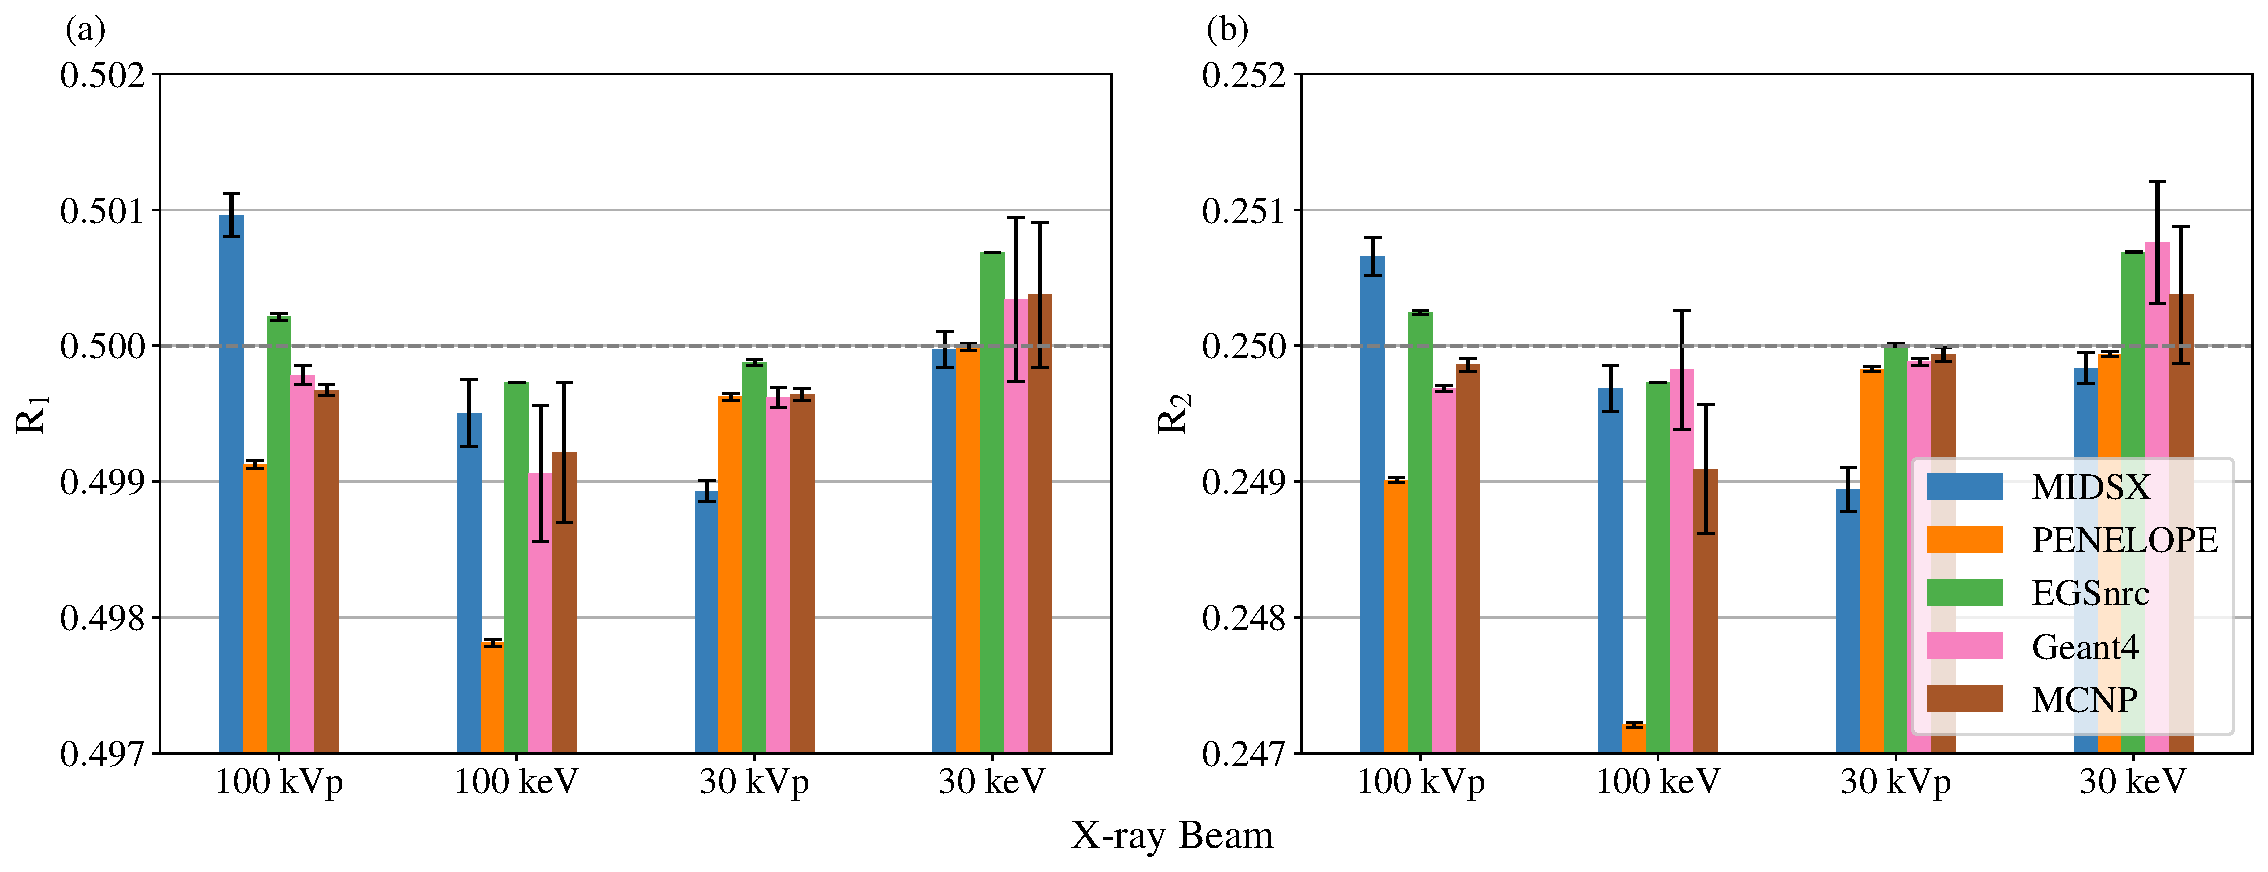
\includegraphics[width=1.0\textwidth]{../figures/HVL_and_QVL_paper_ready.pdf}
	\caption{Results for the (a) HVL and (b) QVL simulations as described by Case 1. The ratios of the primary HVL and QVL air kermas to the primary background air kermas is represented by $R_1$ and $R_2$, respectively. The simulation was performed for the monoenergetic energies 30 keV and 100 keV, along with the polyenergetic spectrums of 30 kVp and 100 kVp, which were provided by TG-195.}
	\label{fig:HVLGraph}
\end{figure}

\begin{figure}[H]
    \centering
	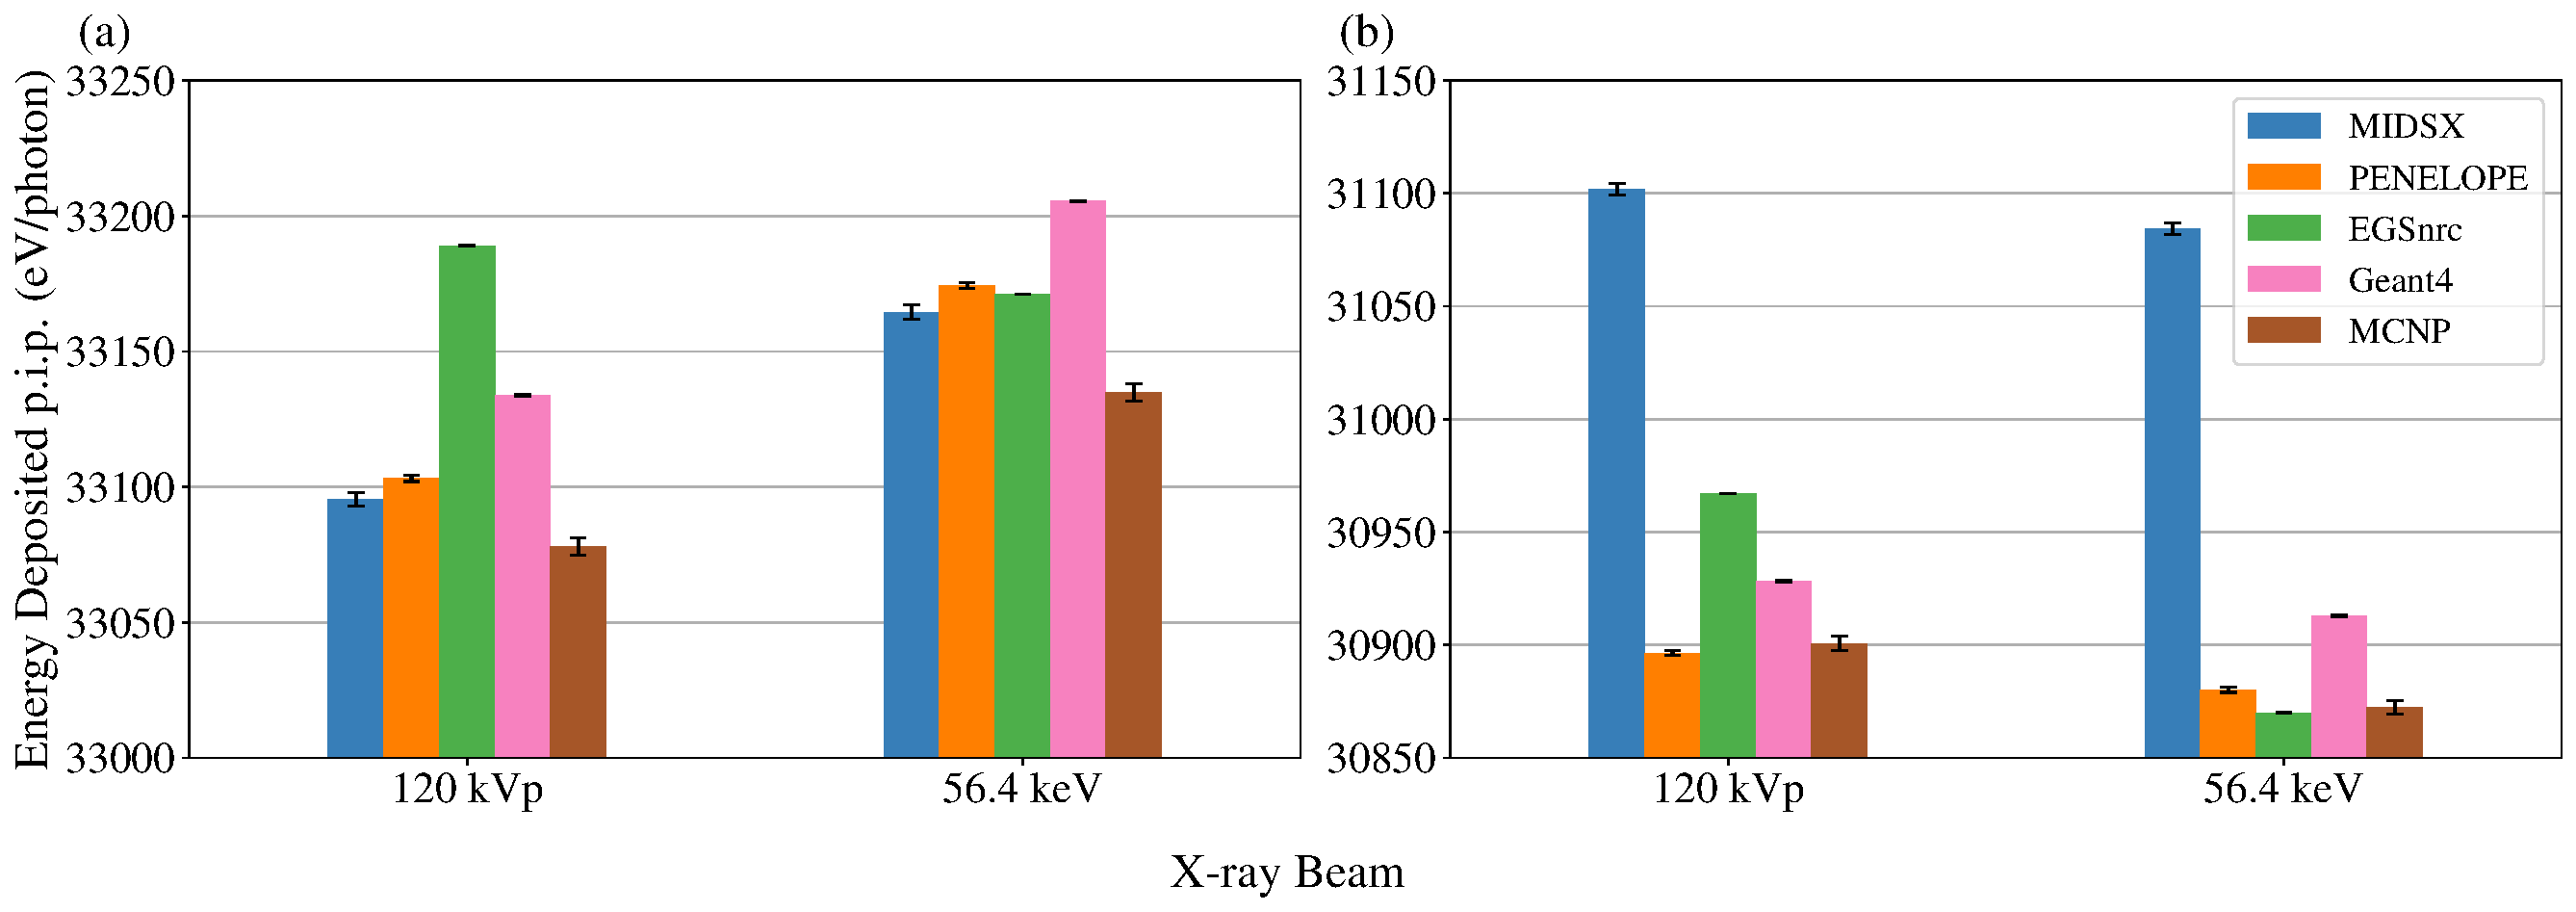
\includegraphics[width=1.0\textwidth]{../figures/radiography_body_dep_paper_ready.pdf}
	\caption{The energy deposited per initial photon (eV/photon) in the simulated tissue for the full-field simulation as described by Case 2. The simulation was performed at 56.4 keV and 120 kVp at both (a) $0^\circ$ and (b) $15^\circ$, with the 120 kVp spectrum provided by TG-195.}
 	\label{fig:BDGraph}
\end{figure}


\FloatBarrier


% \begin{figure}[htbp!]
%     \centering
% 	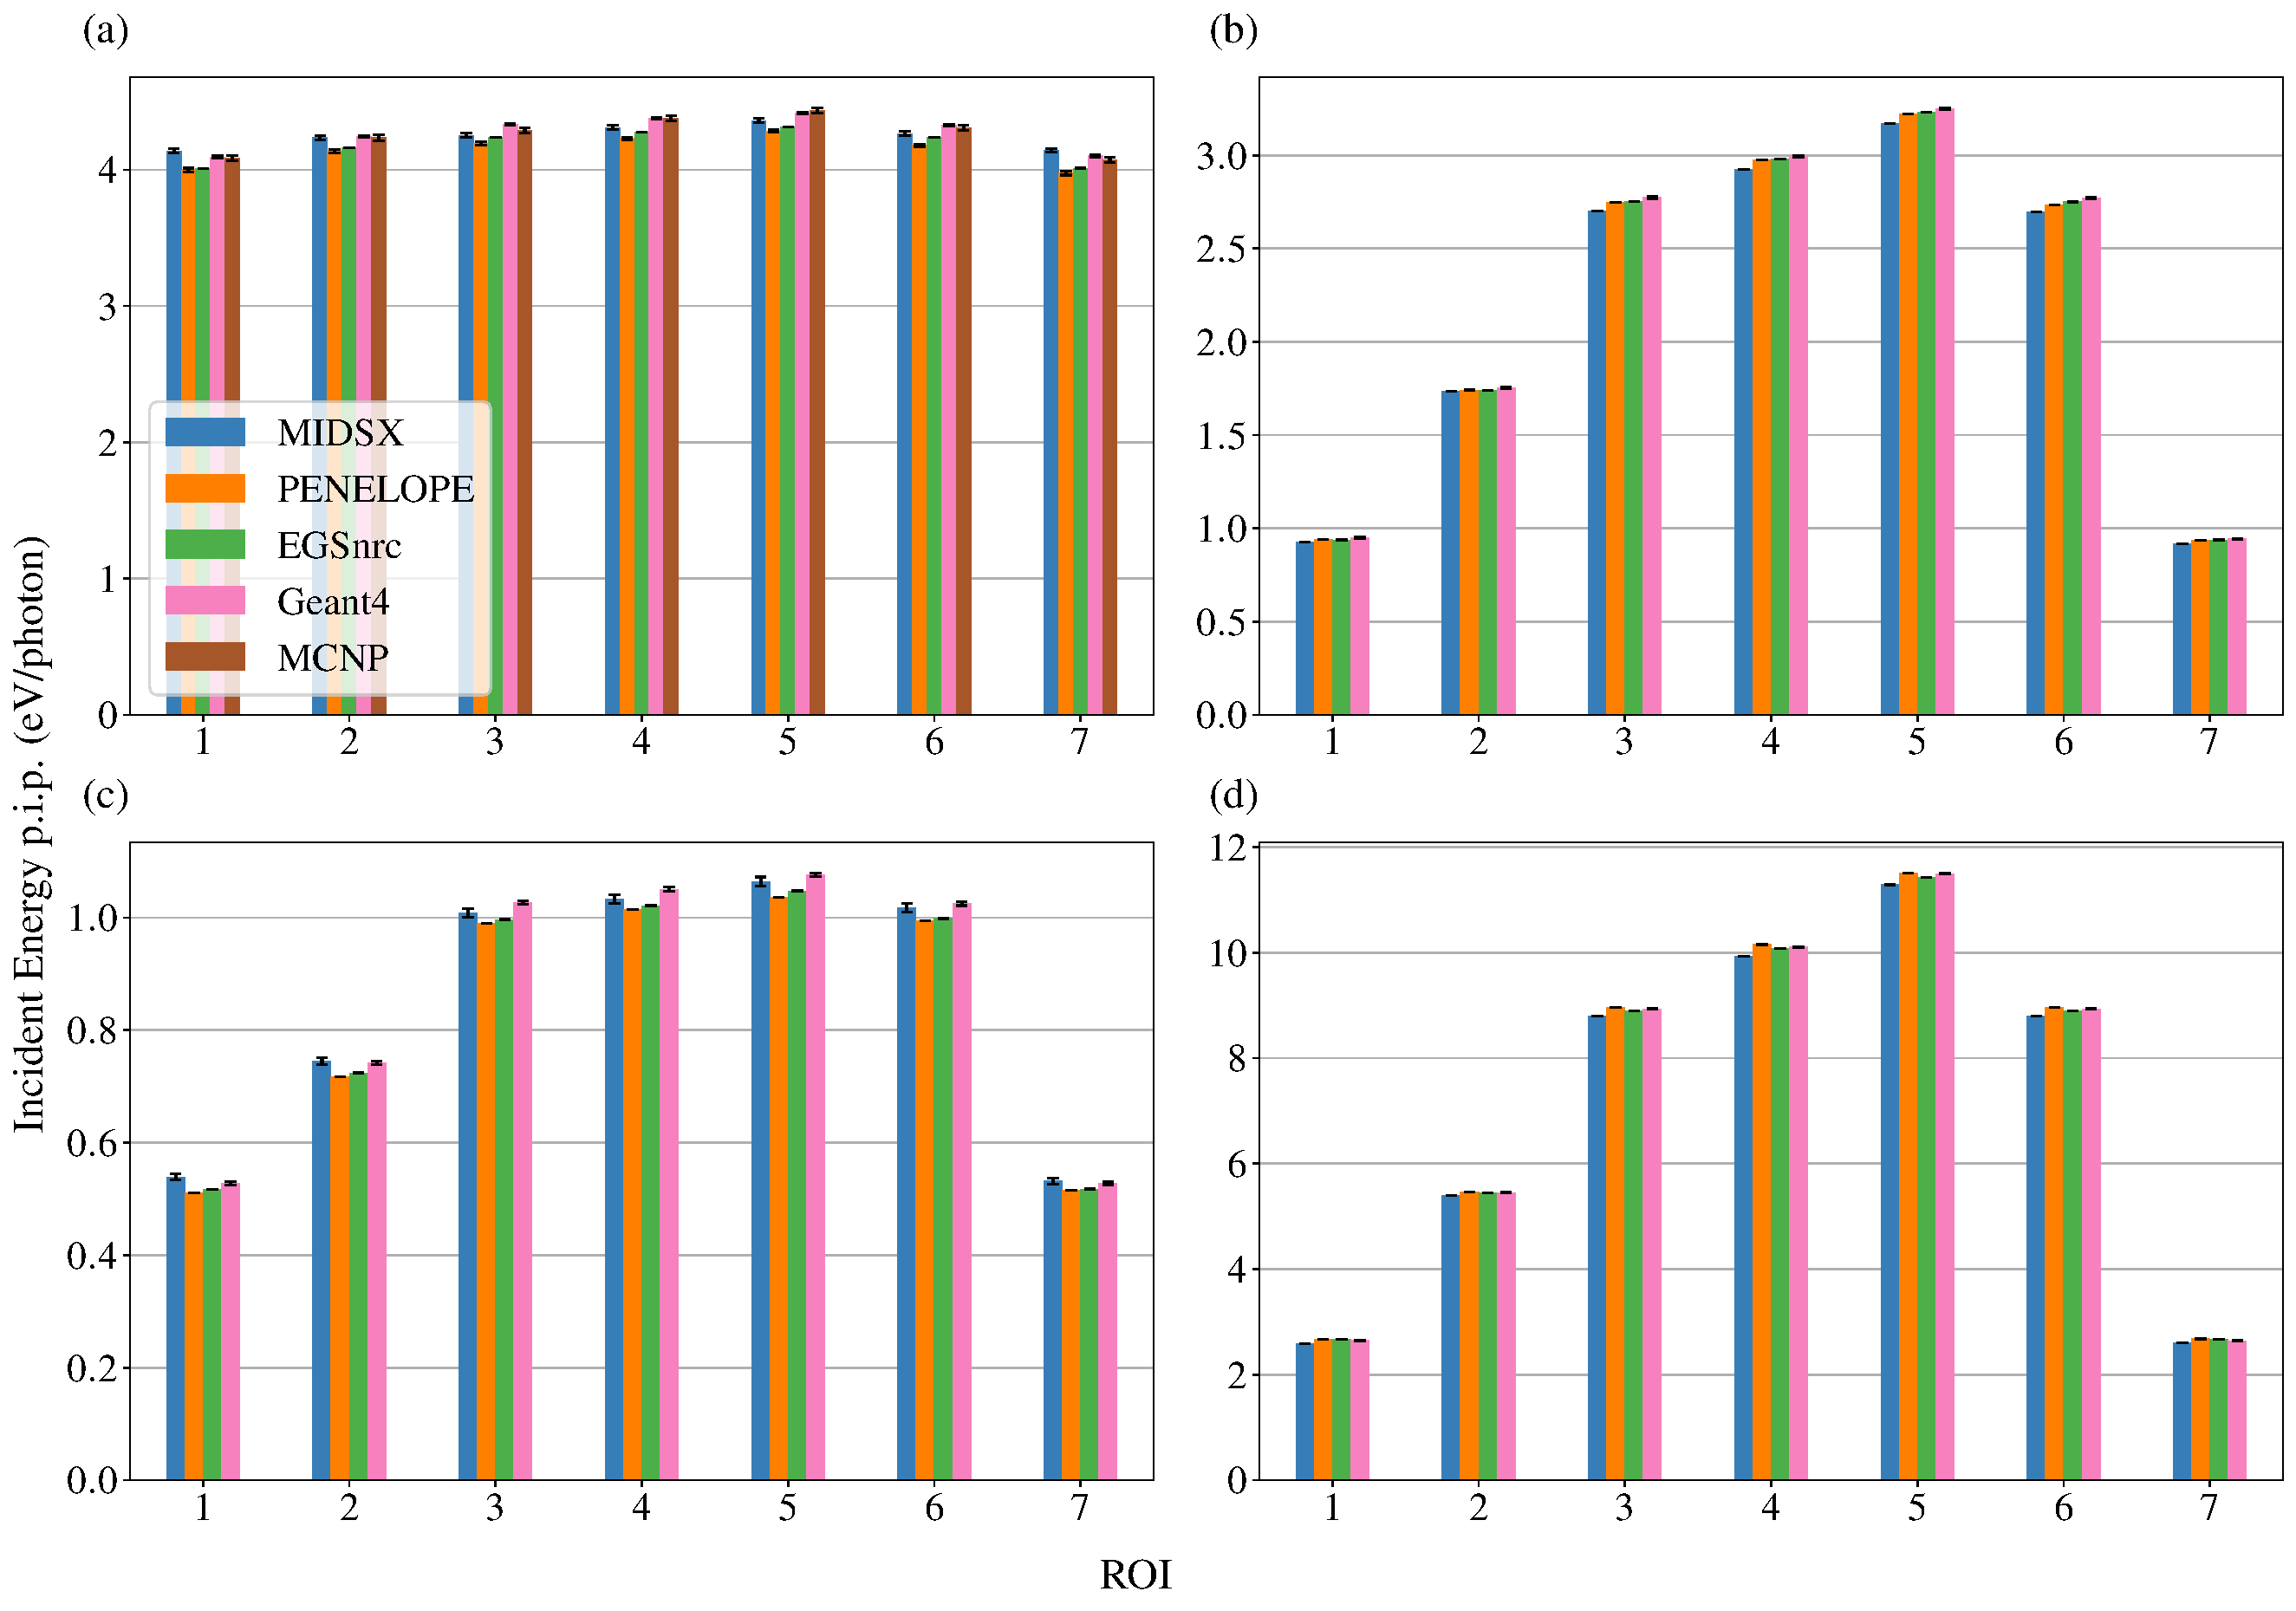
\includegraphics[width=1.0\textwidth]{../figures/ROI_0_deg_paper_ready.pdf}
% 	\caption{The energy per initial photon (eV/photon) of photons incident upon each region of interest (ROI) for the $0^\circ$, full-field, 56.4 keV simulation as described by Case 2. The incident energy was determined separately for photons that underwent (a) no real interactions, (b) a single incoherent scatter, (c) a single coherent scatter, (d) and multiple scatters.}
% 	\label{fig:ROIFFGraph}
% \end{figure}

\begin{figure}[htpb]
    \centering
	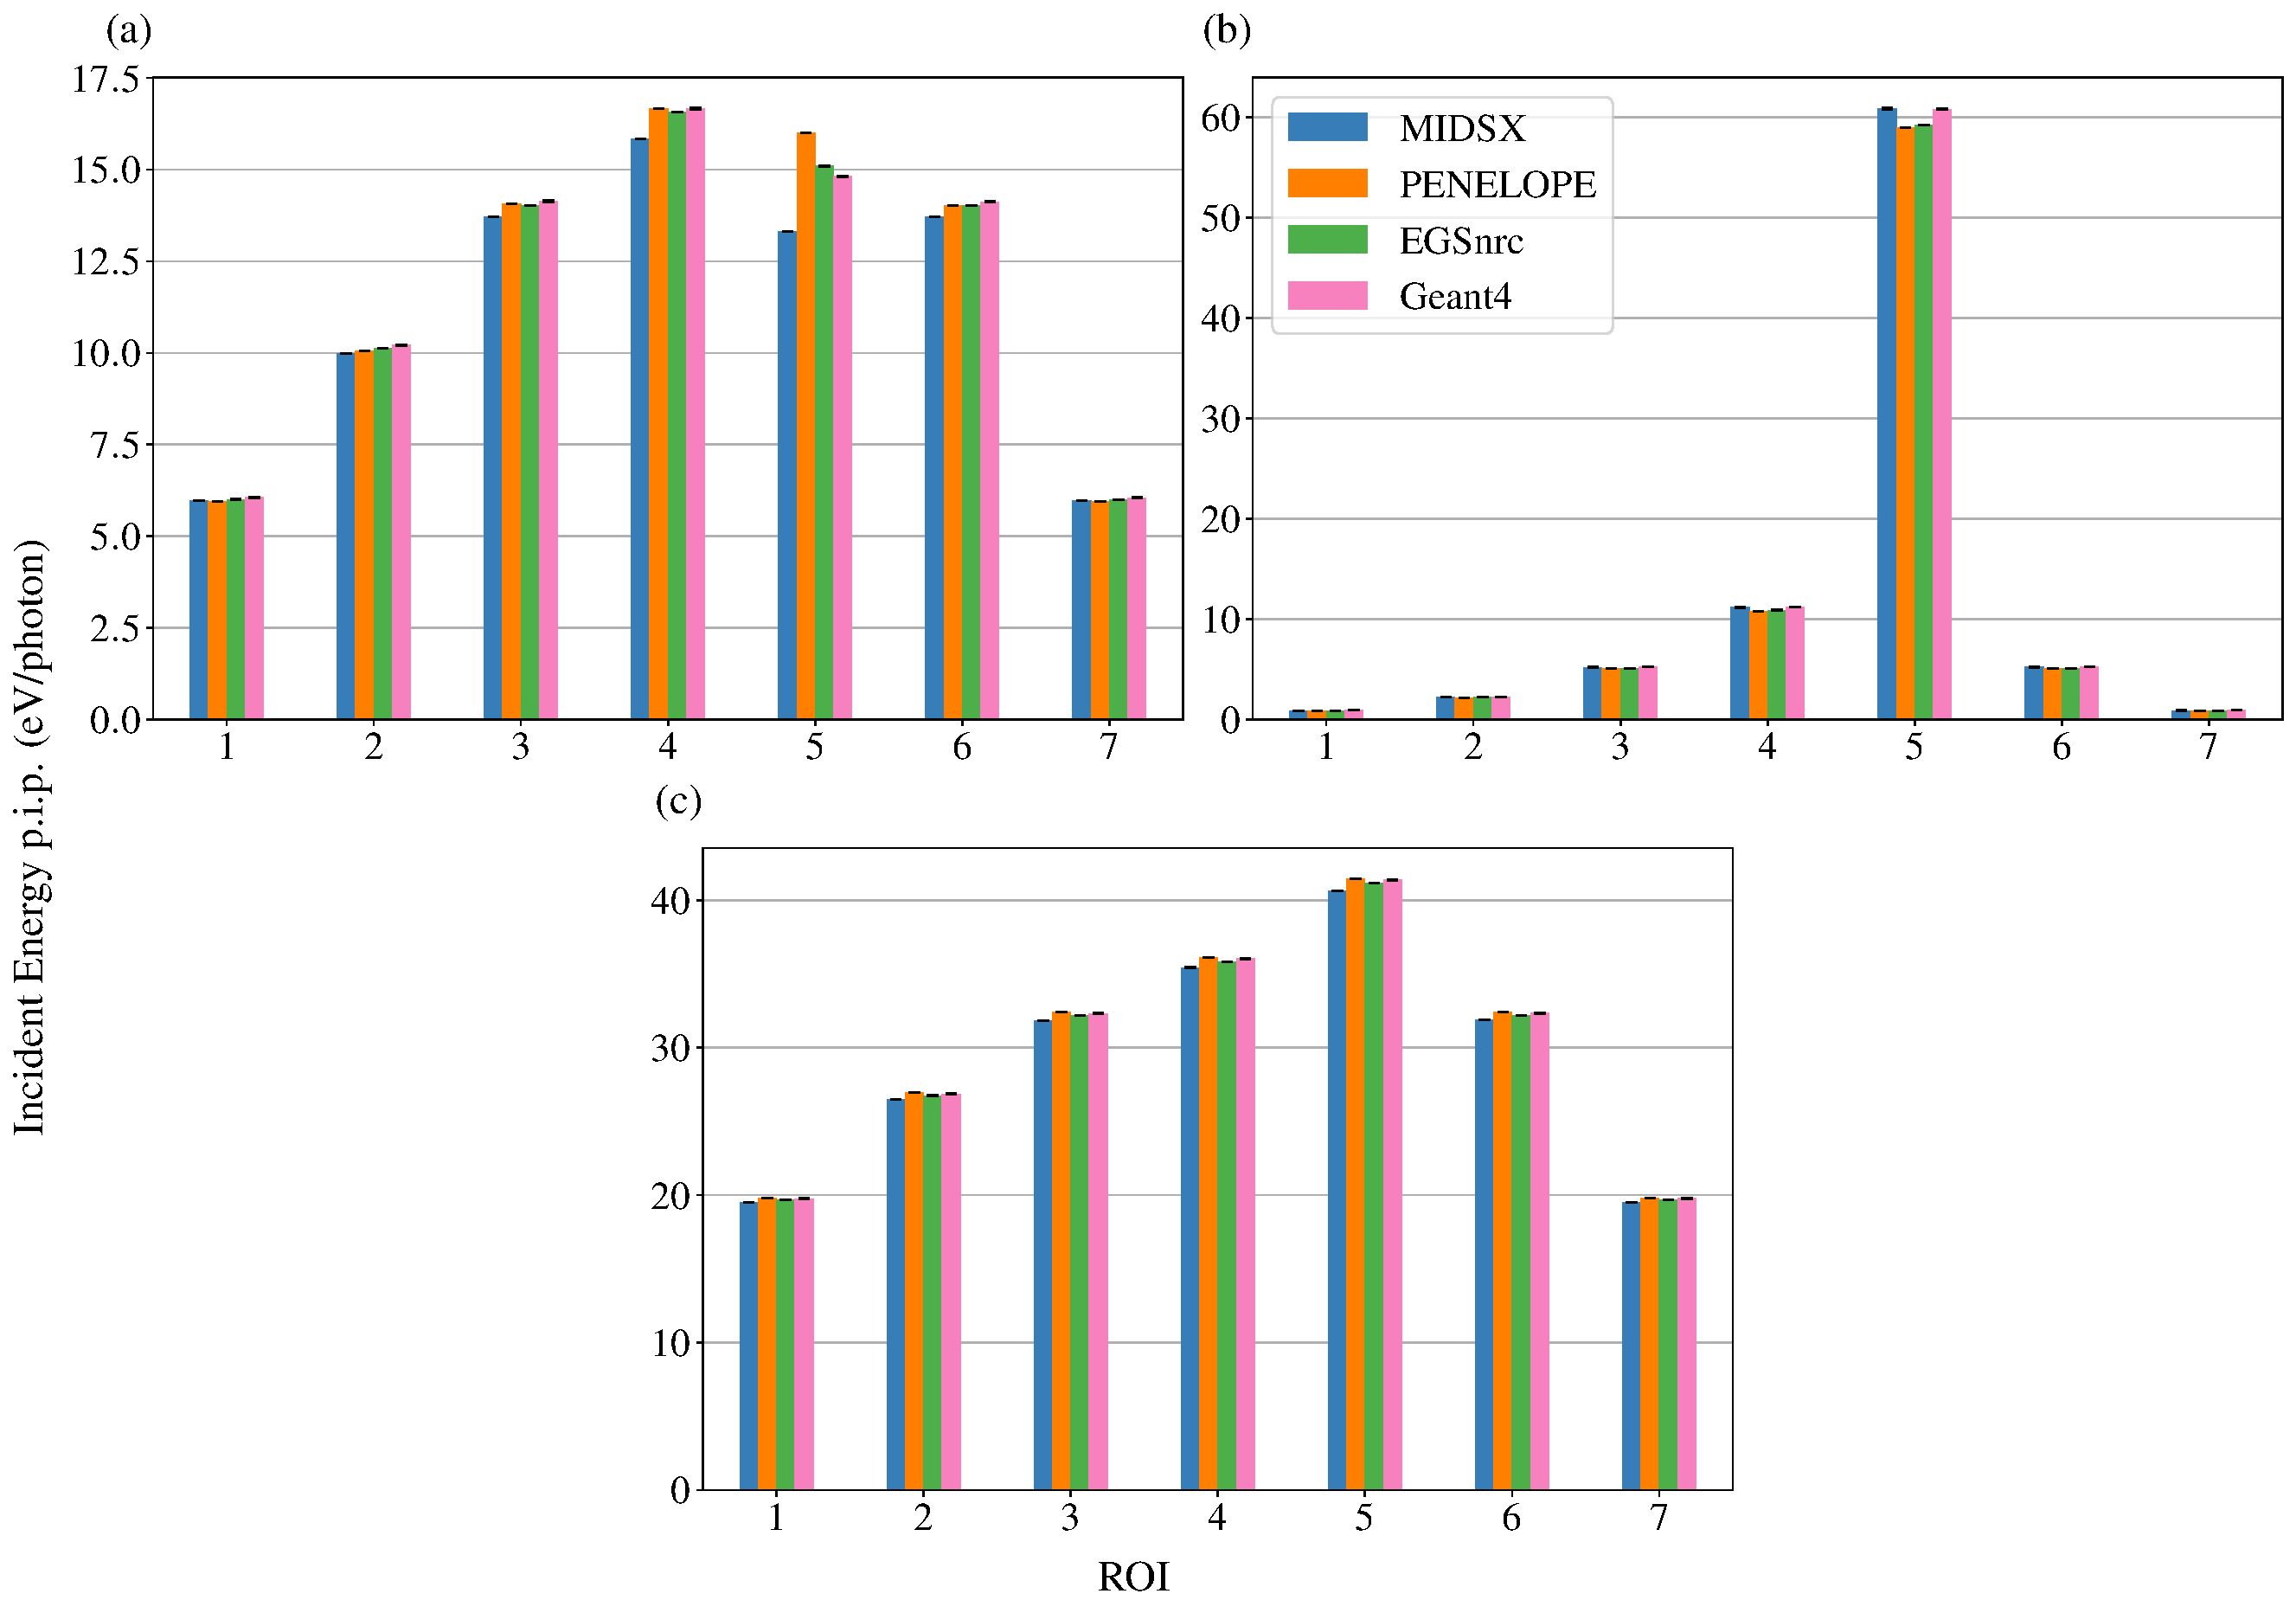
\includegraphics[width=1.0\textwidth]{../figures/ROI_0_deg_pencil_paper_ready.pdf}
	\caption{The energy per initial photon (eV/photon) of photons incident upon each region of interest (ROI) for the $0^\circ$, pencil beam, 56.4 keV simulation as described by Case 2. The incident energy was determined separately for photons that underwent (a) a single incoherent scatter, (b) a single coherent scatter, (c) and multiple scatters.}
	\label{fig:ROIPGraph}
\end{figure}

% \begin{figure}[H]
%     \centering
% 	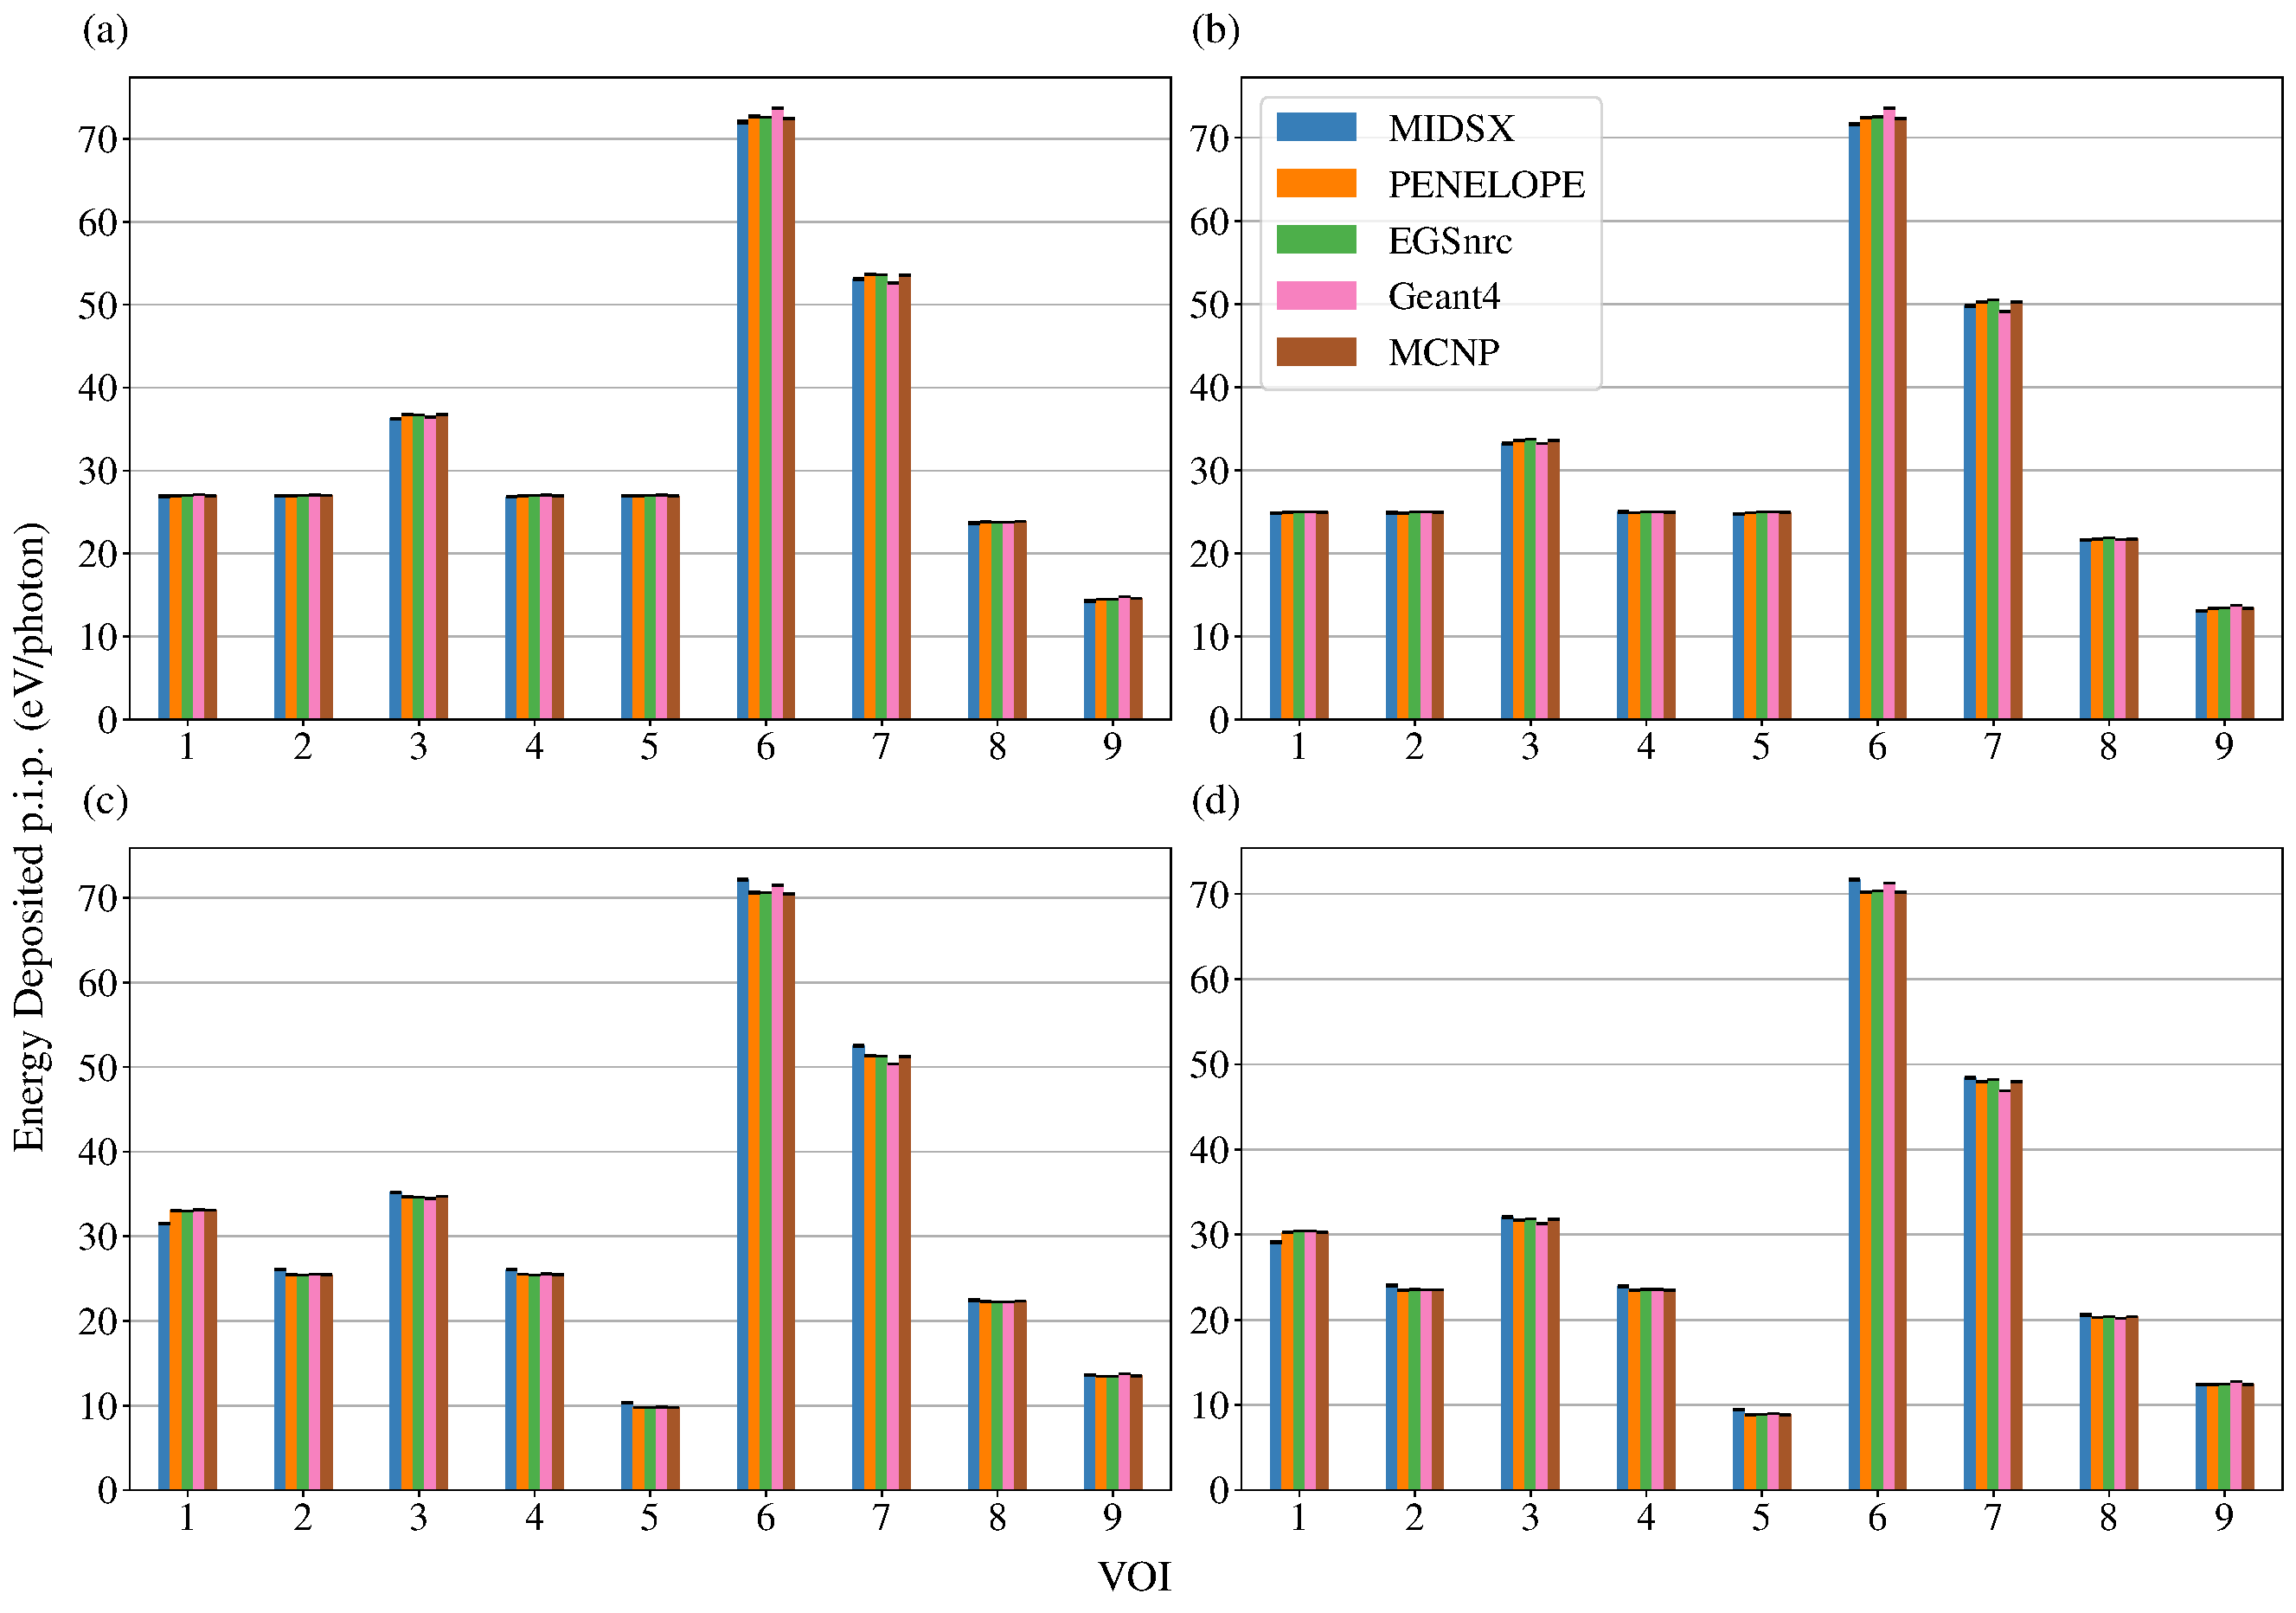
\includegraphics[width=1.0\textwidth]{../figures/VOI_paper_ready.pdf}
% 	\caption{The energy deposited per initial photon (eV/photon) in the volumes of interests (VOIs) for the full field simulation as described by Case 2. The simulation was performed at (a) $0^\circ$/56.4 keV, (b) $0^\circ$/120 kVp, (c) $15^\circ$/56.4 keV, and (d) $15^\circ$/120 kVp.}
% 	\label{fig:VOIFFGraph}
% \end{figure}

% \begin{figure}[H]
%     \centering
% 	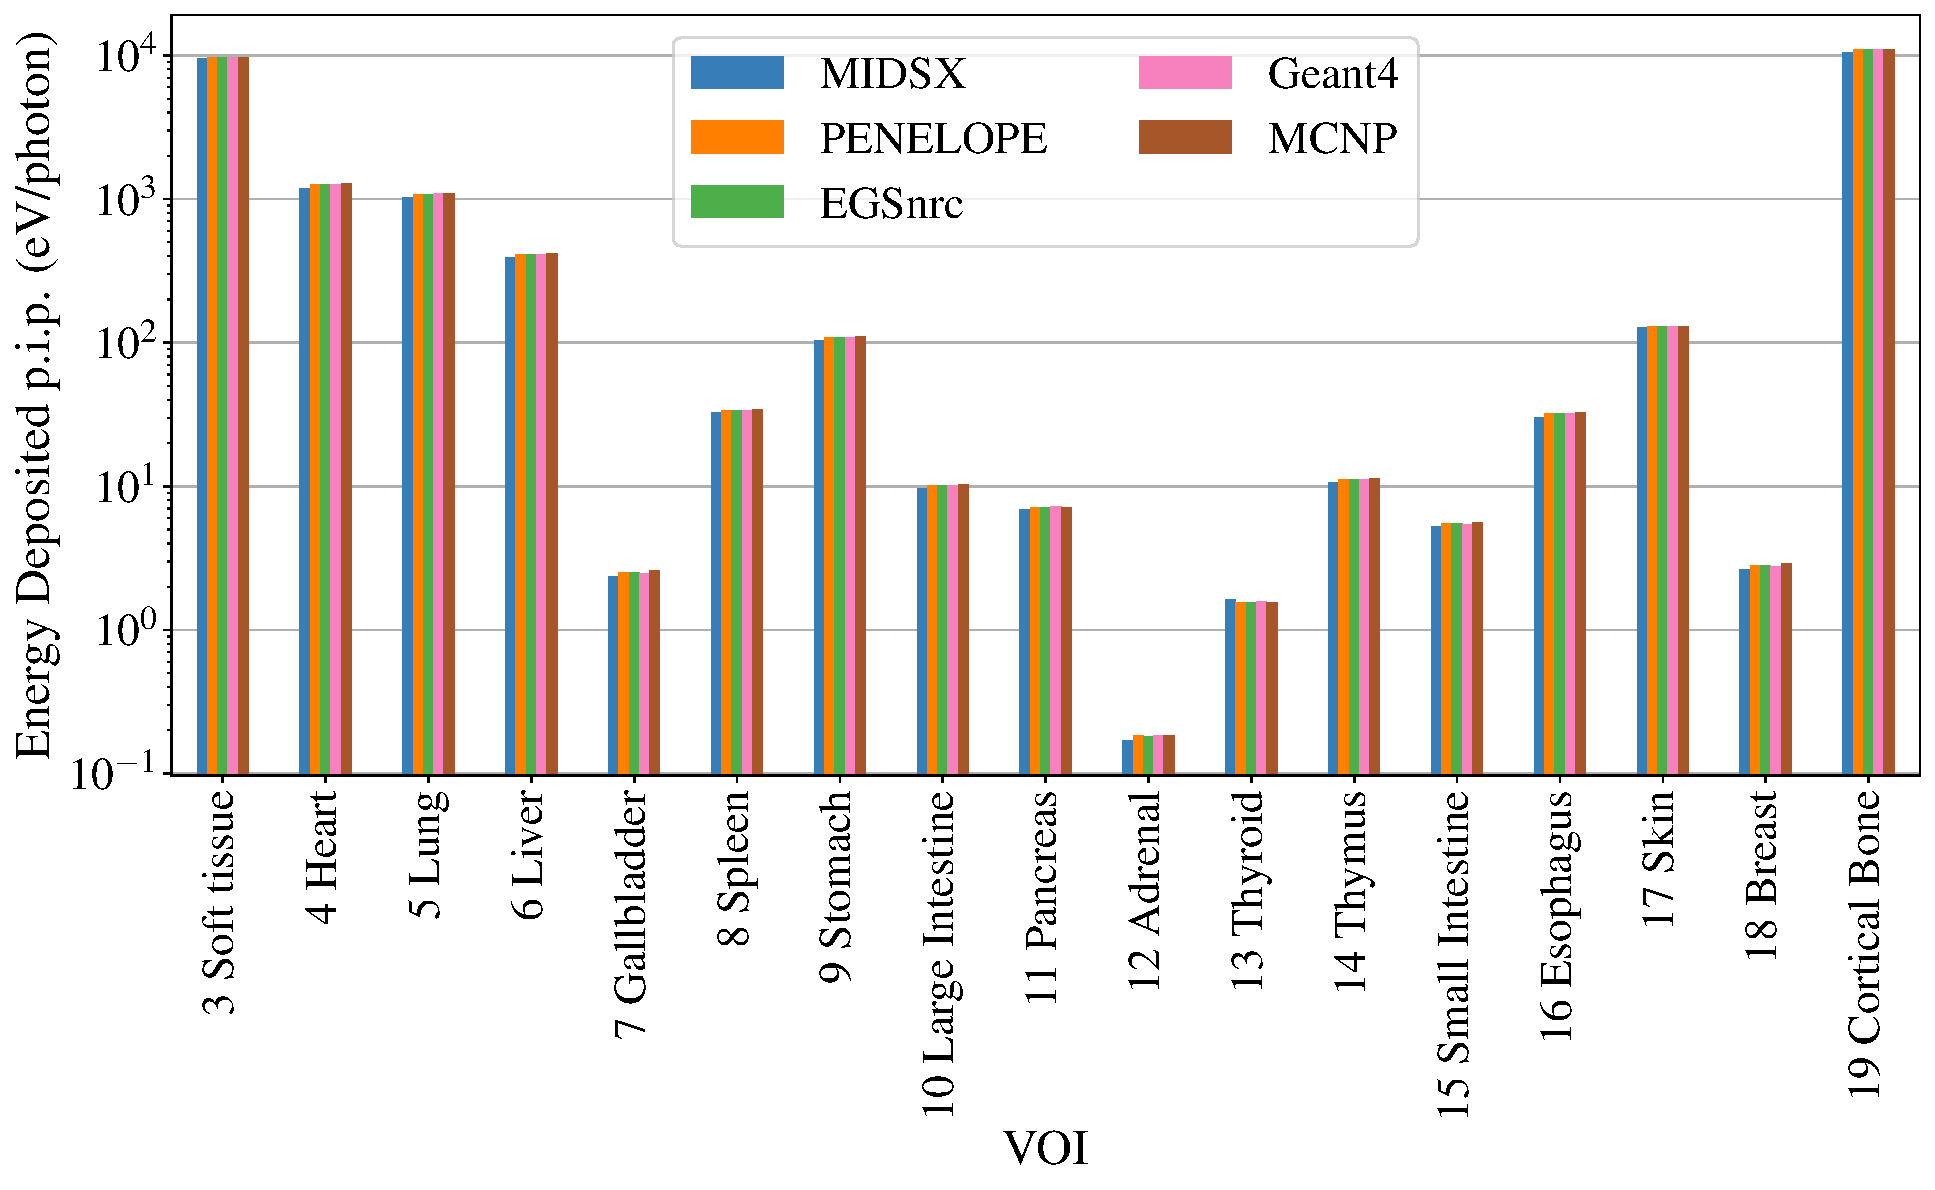
\includegraphics[width=1.0\textwidth]{../figures/CT_564_180.pdf}
% 	\caption{The energy deposited per initial photon (eV/photon) in the material IDs for the $180^\circ$, 56.4 keV simulation as described by Case 5.}
% 	\label{fig:CTGraph}
% \end{figure}

\begin{figure}[htbp]
    \centering
	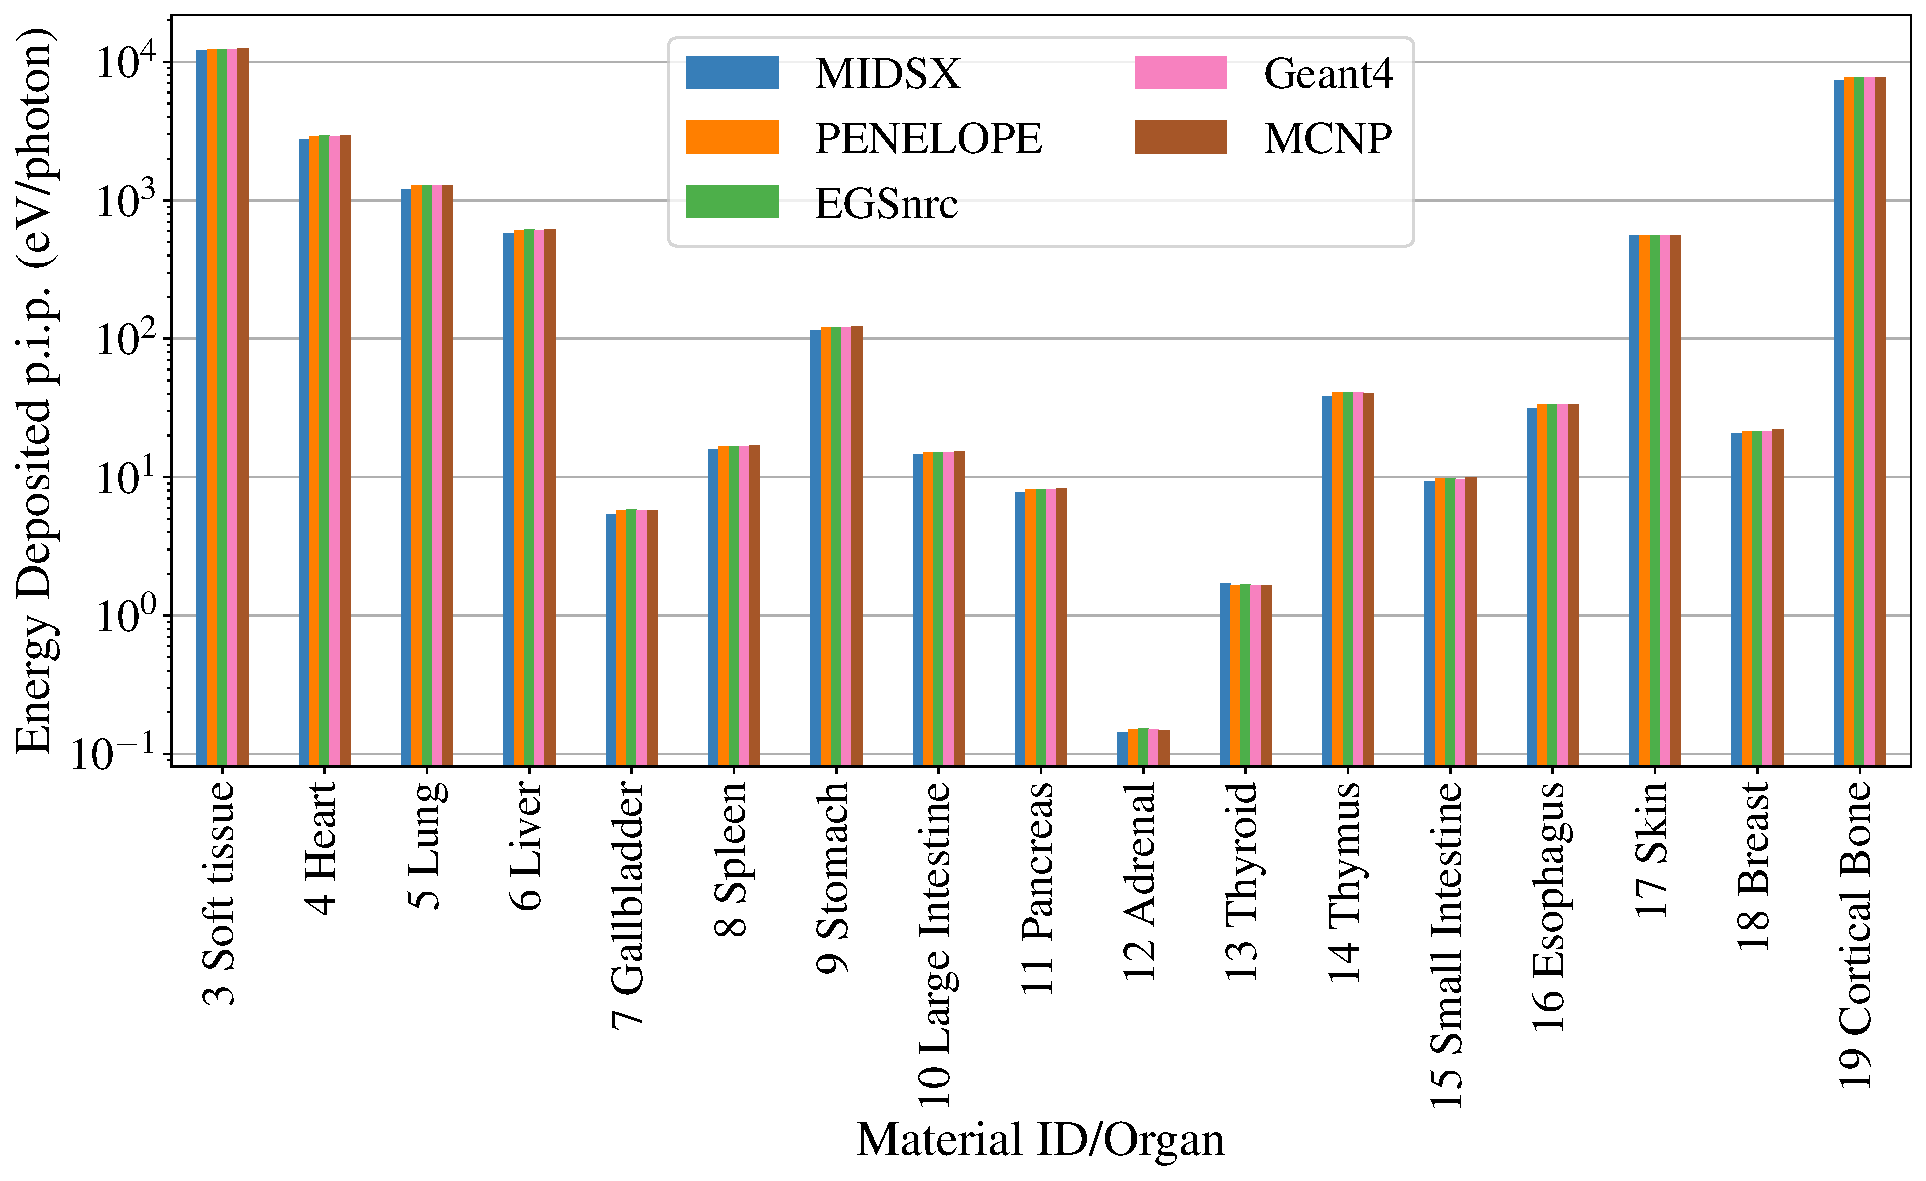
\includegraphics[width=1.0\textwidth]{../figures/CT_120_0.pdf}
	\caption{The energy deposited per initial photon (eV/photon) in the material IDs for the $0^\circ$, 120 kVp simulation as described by Case 5.}
	\label{fig:CTGraph}
\end{figure}

\FloatBarrier
